\chapter{\IfLanguageName{dutch}{Stand van zaken}{State of the art}}%
\label{ch:stand-van-zaken}

% Tip: Begin elk hoofdstuk met een paragraaf inleiding die beschrijft hoe
% dit hoofdstuk past binnen het geheel van de bachelorproef. Geef in het
% bijzonder aan wat de link is met het vorige en volgende hoofdstuk.

% Pas na deze inleidende paragraaf komt de eerste sectiehoofding.

% Dit hoofdstuk bevat je literatuurstudie. De inhoud gaat verder op de inleiding, maar zal het onderwerp van de bachelorproef *diepgaand* uitspitten. De bedoeling is dat de lezer na lezing van dit hoofdstuk helemaal op de hoogte is van de huidige stand van zaken (state-of-the-art) in het onderzoeksdomein. Iemand die niet vertrouwd is met het onderwerp, weet nu voldoende om de rest van het verhaal te kunnen volgen, zonder dat die er nog andere informatie moet over opzoeken \autocite{Pollefliet2011}.

% Je verwijst bij elke bewering die je doet, vakterm die je introduceert, enz.\ naar je bronnen. In \LaTeX{} kan dat met het commando \texttt{$\backslash${textcite\{\}}} of \texttt{$\backslash${autocite\{\}}}. Als argument van het commando geef je de ``sleutel'' van een ``record'' in een bibliografische databank in het Bib\LaTeX{}-formaat (een tekstbestand). Als je expliciet naar de auteur verwijst in de zin (narratieve referentie), gebruik je \texttt{$\backslash${}textcite\{\}}. Soms is de auteursnaam niet expliciet een onderdeel van de zin, dan gebruik je \texttt{$\backslash${}autocite\{\}} (referentie tussen haakjes). Dit gebruik je bv.~bij een citaat, of om in het bijschrift van een overgenomen afbeelding, broncode, tabel, enz. te verwijzen naar de bron. In de volgende paragraaf een voorbeeld van elk.

% \textcite{Knuth1998} schreef een van de standaardwerken over sorteer- en zoekalgoritmen. Experten zijn het erover eens dat cloud computing een interessante opportuniteit vormen, zowel voor gebruikers als voor dienstverleners op vlak van informatietechnologie~\autocite{Creeger2009}.

% Let er ook op: het \texttt{cite}-commando voor de punt, dus binnen de zin. Je verwijst meteen naar een bron in de eerste zin die erop gebaseerd is, dus niet pas op het einde van een paragraaf.

% \lipsum[7-20]

% Change detection
\section{\IfLanguageName{dutch}{Remote Sensing Change Detection}{Remote Sensing Change Detection}}%
\label{sec:remote-sensing-change-detection}

Remote sensing change detection (RSCD) is het waarnemen van verandering in een bepaald gebied aan de hand van op afstand genomen afbeeldingen op
verschillende tijdstippen \autocite{SINGH_1989}. Data bestaat meestal uit lucht- of satellietfoto’s. Gebruikte applicaties zijn onder meer het 
monitoren van ontbossing of de impact van natuurrampen bestuderen.
\newline
CD kan onder menselijke toezicht gebeuren door de twee foto's naast elkaar te leggen en zo de verschillen te zoeken. 
Na de opkomst van computers werden verschillende nieuwe methodes uitgevonden. Single-pixel methoden zoals image difference \autocite{QUARMBY_1989} 
en image ratio \autocite{HOWARTH_1981}. Andere bekende methode zijn principle component analysis \autocite{Deng_2008} en change vector analysis \autocite{Carvalho_J_nior_2011}. 
Rond de jaren 90, na de opkomst van computer vision, begon er ook binnen RSCD use cases te onstaan. Dit wordt aangetoond in studies zoals
\textcite{levien1999machine} en \textcite{dai1999remotely}. 
Sindsdien is er een groepering van traditionele en AI gebaseerde technieken ontstaan. Over de jaren heen zijn computer vision 
modellen alsmaar complexer geworden. Verschillende recente studies zoals \textcite{zerrouki2019machine} tonen aan dat machine learning algoritmen 
beter en efficiënter zijn in RSCD dan de traditionele methodes. 
\newline
\newline

% Remote sensing change detection (CD) verwijst naar het proces van het identificeren en analyseren van veranderingen in een 
% specifiek gebied op basis van afbeeldingen die op verschillende tijdstippen zijn genomen \autocite{SINGH_1989}. 
% Landschappelijke veranderingen kunnen significante gevolgen hebben voor zowel het klimaat als de leefomstandigheden van mens en dier. 
% Het systematisch monitoren van deze veranderingen is van cruciaal belang om potentiële problemen tijdig te signaleren en gepaste 
% maatregelen te nemen. Dit onderzoek richt zich specifiek op de aanwezigheid van vegetatie in een stedelijke omgeving.
% Traditioneel kan CD worden uitgevoerd door visuele inspectie, waarbij beelden uit verschillende tijdstippen naast elkaar worden gelegd 
% om verschillen te detecteren. Uit diverse onderzoeken zoals \textcite{zerrouki2019machine} blijkt echter dat machine learning-algoritmen aanzienlijk effectiever en 
% efficiënter zijn in het geautomatiseerd herkennen van veranderingen in het landschap.
% \newline
% \newline

% Computer vision
\section{\IfLanguageName{dutch}{Computer Vision}{Computer Vision}}%
\label{sec:computer-vision}

Computer vision is een onderdeel van artificiële intelligentie (AI) dat zich richt op het werken met visuele data (foto's, video's enz\ldots) 
\autocite{ibm2025b}. Het bekendste voorbeeld hiervan is foto classificatie. Een algoritme dat een gegeven foto kan classificeren tot een 
bepaalde klasse. Lange tijd was, deze op eerste zicht simpele taak, niet op betrouwbare wijze uit te voeren door machine learning \autocite{Geron2022}.
Met de opkomst van deep learning (DL) en het convolutionele neurale netwerk (CNN) is er in de laatste decennia veel vooruitgang geboekt
in dit veld. De eerste grote doorbraak kwam in 2012 met de overwinning van AlexNet in de ImageNet-competitie \autocite{krizhevsky2012imagenet}. 
Door de beschikbaarheid van grootschalige datasets (zoals COCO en ImageNet), verhoogde rekenkracht en nieuwe architecturen 
blijft het veld constant evolueren.

% De methode die voor dit onderzoek gebruikt zal worden is semantische segmentatie.


% Computer vision is een subdiscipline binnen de artificiële intelligentie (AI) die zich richt op het automatisch interpreteren, 
% begrijpen en extraheren van informatie uit visuele input, zoals foto's, video's of beelden afkomstig van sensoren \autocite{ibm2025b}. 
% Het doel van computer vision is om computers in staat te stellen visuele data op een manier te analyseren die vergelijkbaar is met, 
% of zelfs beter dan, de menselijke waarneming.
% \newline
% \newline
% Een van de meest fundamentele taken binnen computer vision is beeldclassificatie, waarbij een algoritme een afbeelding analyseert en deze toewijst aan 
% een vooraf gedefinieerde klasse, zoals "kat", "auto", of "boom". Hoewel dit op het eerste gezicht een eenvoudige taak lijkt, vormde het jarenlang een 
% grote uitdaging voor traditionele machine learning-methoden, die afhankelijk waren van handmatig geëxtraheerde kenmerken en beperkt waren in 
% hun generaliseerbaarheid \autocite{Geron2022}.
% \newline
% \newline
% De doorbraak in dit domein kwam met de opkomst van deep learning, en in het bijzonder convolutionele neurale netwerken (CNN's). 
% CNN's zijn in staat om automatisch ruimtelijke hiërarchieën van kenmerken te leren, waardoor ze uitblinken in het verwerken van visuele patronen \autocite{LeCun_2015}. 
% Sinds de overwinning van AlexNet op de ImageNet-competitie in 2012 \autocite{krizhevsky2012imagenet}, 
% zijn CNN-gebaseerde modellen de dominante benadering geworden voor talrijke computer vision-toepassingen, waaronder objectdetectie, beeldsegmentatie, 
% gezichtsherkenning en actieherkenning in video.
% \newline
% \newline
% Binnen de context van dit onderzoek ligt de focus op \textit{semantische segmentatie}, een taak die verder gaat dan eenvoudige classificatie. 
% Hierbij wordt elk afzonderlijk pixel in een afbeelding geclassificeerd als behorend tot een specifieke semantische categorie. 
% Deze fijnmazige benadering is essentieel in domeinen waar ruimtelijke precisie en context cruciaal zijn, zoals in medische beeldanalyse, 
% autonome voertuigen en satellietbeelden voor stedelijke en ecologische monitoring \autocite{zhu2017deep}.
% \newline
% \newline
% De recente vooruitgang in computer vision wordt mede mogelijk gemaakt door beschikbaarheid van grootschalige datasets (zoals ImageNet en COCO), 
% verhoogde rekenkracht (GPU's en TPU's), en nieuwe architecturen zoals Vision Transformers (ViTs), 
% die gebruik maken van self-attention mechanismen om contextuele informatie effectiever te modelleren \autocite{dosovitskiy2020image}.
% \newline
% \newline

% Semantic Segmentation
% \section{\IfLanguageName{dutch}{Semantische Segmentatie}{Semantic Segmentation}}%
% \label{sec:semantische-segmentatie}

% Semantische segmentatie is een computer vision taak dat elke pixel in een bepaalde klasse classificeerd aan de hand van machine learning 
% modellen \autocite{ibm2025a}. De output vormt een segmentatie kaart. Dit is een kopie van de originele foto waarbij elke pixel tot 
% een bepaalde segmentatie mask behoort. Masks zijn delen van de foto waarbij gelijkaardige pixels samen een object vormen \autocite{Geron2022}.
% Semantische segmentatie wordt bijvoorbeeld gebruikt voor AI sturende voertuigen en camera's om objecten zoals mensen te identificeren \autocite{ibm2025a}. 
% \newline
% \newline

% Semantische segmentatie is een fundamentele taak binnen het domein van computer vision waarbij elk afzonderlijk pixel in een afbeelding wordt geclassificeerd 
% als behorend tot een specifieke semantische klasse, zoals "weg", "vegetatie", "gebouw" of "lucht" \autocite{ibm2025a}. 
% In tegenstelling tot objectdetectie, dat enkel bounding boxes genereert rondom objecten, biedt semantische segmentatie een fijnmazige representatie 
% van objectgrenzen, wat essentieel is voor toepassingen waar precieze lokalisatie van klasse-informatie op pixelniveau vereist is.
% \newline
% \newline
% De output van een semantisch segmentatiemodel is een zogenaamde \textit{segmentatiekaart}, een afbeelding met dezelfde resolutie als de invoerafbeelding, 
% waarbij elke pixel een label draagt dat overeenkomt met de geclassificeerde klasse. Pixels die tot hetzelfde objecttype behoren, 
% vormen samen een \textit{mask}, of segment, wat het mogelijk maakt om objecten van dezelfde klasse consistent te identificeren, 
% ongeacht hun locatie in de afbeelding \autocite{garcia2020review}.
% \newline
% Moderne semantische segmentatiemodellen zijn doorgaans gebaseerd op convolutionele neurale netwerken (CNNs) en encoder-decoder architecturen. 
% De encoder (bijvoorbeeld ResNet of VGG) extraheert hiërarchische kenmerken uit het beeld door middel van convolutielagen, 
% terwijl de decoder deze abstracte representaties herprojecteert naar de originele resolutie met behulp van upsampling of transposed convoluties \autocite{ronneberger2015u}. 
% % Bekende modellen binnen dit domein zijn onder andere FCN (Fully Convolutional Network), U-Net, DeepLabv3+ en SegNet.
% \begin{figure}[h]
%   \caption{Voorbeeld van semantische segmentatie}
%   \centering 
%   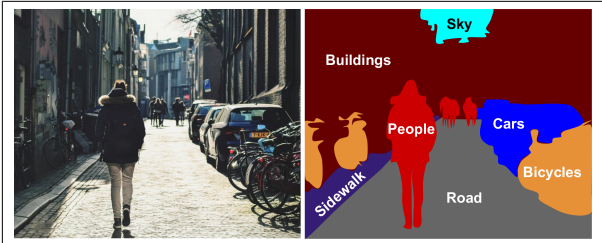
\includegraphics{Sematische Segmentatie.png}
%   \end{figure}
% \newline
% \newline
% Een belangrijk aspect binnen semantische segmentatie is het behouden van ruimtelijke resolutie tijdens de opwaartse reconstructie van de afbeelding. 
% Technieken zoals skip connections (bijvoorbeeld in U-Net) worden gebruikt om fijnmazige kenmerken uit vroege lagen van het netwerk te combineren met 
% de globale contextinformatie van de diepere lagen, wat leidt tot een hogere nauwkeurigheid bij het detecteren van fijne objectranden \autocite{ronneberger2015u}.
% \newline
% In toepassingen zoals medische beeldvorming, autonome voertuigen en remote sensing, is semantische segmentatie een cruciaal hulpmiddel. 
% In remote sensing, bijvoorbeeld, maakt deze techniek het mogelijk om stedelijke infrastructuur, 
% vegetatiezones of waterlichamen op schaal te identificeren vanuit satellietbeelden met hoge resolutie, 
% wat van groot belang is voor milieumonitoring en stedelijke planning \autocite{zhu2017deep}.
% \newline
% \newline

% Machine Learning
\section{\IfLanguageName{dutch}{Machine Learning}{Machine Learning}}%
\label{sec:machine-learning}

Machine learning (ML) is een onderdeel van artificiële intelligentie (AI) gericht op het imiteren van menselijke leerprocessen, dat instaat 
is zelfstandig keuzes te maken aan de hand van training met gerichte data \autocite{ibm2025}. De term werd voor het eerst gebruikt in de 
jaren 50 door Arthur Samuel. Een pionier in de vroege ontwikkeling van AI en ML, meest bekend voor zijn computer model dat in staat 
was om de winkans op elk moment in een match dammen van beide spelers te bereken. 
\newline
\newline
Binnen machine learning heersen verschillende 'learning' technieken. De drie belangrijkste 
zijn supervised, unsupervised en reinforcement learning \autocite{Geron2022}. In dit onderzoek wordt gebruik gemaakt van supervised learning. Het model maakt 
gebruik van gelabelde data. Elke input heeft een gelabelde output. Dit kan manueel gedaan worden door mensen of automatisch aan de 
hand van een bestaand algoritme. Het idee achter gelabelde data is dat het ML model hieruit patronen kan vinden gebaseerd op de input output
relatie. 
\newline
\newline
Een Machine learning model wordt opgedeeld in verschillende stappen. De meest voorkomende zijn preprocessing, training en evaluatie.
Samen vormen ze een ML pipeline. Het preprocessing deel bevat operaties die op de data moeten worden uitgevoerd voordat de training van 
start kan gaan. Veel voorkomende technieken zijn data normalisatie, data herschalen enz \ldots. De trainingsfase behoud zich tot het
trainen van de data. Het model krijgt input (data) binnen en moet op basis van deze input een output geven. Bij supervised learning bevat
de input ook al de gewenste output (labels). De labeling kan handmatig worden uitgevoerd door menselijke annotators of 
automatisch worden gegenereerd door een bestaand algoritme.
\newline
\newline
Het doel van ML training is om het model te leren zelfstandig beslissingen te maken op basis van de input data. 
Wanneer een model voldoende getraind is, wordt het geëvalueerd met nieuwe, ongeziene data. De evaluatie is
vergelijkbaar met de trainingsfase met als verschil dat er nu geen labels worden meegegeven. Het model moet nu zelf de output voorspellen.
Tijdens de evaluatie worden een aantal beoordeling criteria gebruikt. De accuraatheid van het model (procent van output die overeenkomt met
label) bijvoorbeeld. Na de evaluatie wordt het model hertraind als de statistieken niet hoog genoeg zijn. Wanneer de evaluatie criteria behaald 
zijn kan het model gebruikt worden in een productie omgeving.
\newline
\newline

% Machine learning (ML) is een subdiscipline binnen artificiële intelligentie (AI) die zich richt op het nabootsen van menselijke 
% leerprocessen en in staat is om zelfstandig beslissingen te nemen op basis van training met gerichte datasets \autocite{ibm2025}. 
% De term `machine learning' werd voor het eerst geïntroduceerd in de jaren 1950 door Arthur Samuel, een pionier op het gebied van AI en ML, 
% die vooral bekend werd door zijn schaakprogramma dat de winstkansen van beide spelers kon berekenen. Er zijn twee soorten machine learning
% taken: classificatie en regressie. Bij classificatie behoord de output van het model tot een gedefineerde klasse. Bij regressie is de 
% output meer variabel. Meestal een float of integer waarde.
% \newline
% \newline
% Binnen machine learning bestaan ook verschillende leermethoden, waarvan de drie belangrijkste supervised-, unsupervised- en 
% reinforcement learning zijn. In dit onderzoek wordt gebruikgemaakt van supervised learning, een methode waarbij het model wordt getraind 
% met gelabelde data \autocite{mahesh2020machine}. Dit betekent dat elke input in de trainingsset correspondeert met een bekende, vooraf bepaalde output. 
% De labeling kan handmatig worden uitgevoerd door menselijke annotators of automatisch worden gegenereerd door een bestaand algoritme. 
% Het doel van gelabelde data is het identificeren van patronen in de input-output relatie, zodat het model zelfstandig voorspellingen kan 
% doen op basis van nieuwe gegevens.
% \newline
% \newline
% Een machine learning-model wordt doorgaans ontwikkeld in verschillende fasen, die samen een ML-pijplijn vormen. 
% De meest voorkomende stappen zijn preprocessing, training en evaluatie. De preprocessingfase omvat verschillende operaties die 
% noodzakelijk zijn om de ruwe data geschikt te maken voor training \autocite{Geron2022}. Veelgebruikte technieken in deze fase zijn data-normalisatie en rescaling.
% Tijdens de trainingsfase wordt het model getraind door middel van inputdata, waarbij het leert om de bijbehorende output te voorspellen. 
% In het geval van supervised learning betekent dit dat zowel de invoer als de gewenste uitvoer (labels) beschikbaar zijn. 
% Het doel van deze fase is het optimaliseren van het model zodat het zelfstandig beslissingen kan nemen op basis van nieuwe invoergegevens.
% Na de trainingsfase wordt het model geëvalueerd met nieuwe, ongeziene data. In deze evaluatiefase ontvangt het model enkel input, 
% zonder bijbehorende labels, en moet het zelfstandig een output genereren. De prestaties van het model worden beoordeeld aan de hand 
% van verschillende maatstaven, zoals nauwkeurigheid (het percentage correcte voorspellingen ten opzichte van de labels). 
% Indien de prestaties onvoldoende zijn, wordt het model opnieuw getraind en geoptimaliseerd totdat de evaluatiecriteria zijn behaald. 
% Zodra het model voldoet aan de gestelde eisen, kan het worden ingezet in een productieomgeving.
% \newline
% \newline

% Deep learning & Neurale netwerken
\section{\IfLanguageName{dutch}{Deep Learning en Neurale Netwerken}{Deep learning and Neural Networks}}%
\label{sec:deep-learning-neurale-netwerken}

Deep learning is een sub discipline van machine learning dat zich focust op artificiële neurale netwerken (ANN) \autocite{Geron2022}. 
ANN is, zoals de naam aangeeft, een model gebaseerd op de neurale netwerken van het menselijke brein. In 1943 werd in het onderzoek van 
\textcite{McCulloch1943} een artificiële neuron voorgesteld. Gelijkaardig aan biologische neuronen worden artificiële neuronen 
geactiveerd door (binaire) inputs. Dit maakt ze instaat om logische berekeningen op te lossen zoals het AND en OR logische probleem. 
\newline
\newline
De volgende doorbraak kwam in 1958 met het onderzoek van \textcite{Rosenblatt1958} met de preceptron. 
Rosenblatt maakte een nieuwe versie van de artificiële neuron genaamd threshold logic unit (TLU). 
De neuron heeft een set van weights op al de inputs plus één bias term.
Deze berekeningen worden gevolgd door twee activatie functies. Eerst een lineaire functie op alle inputs: \( w^t x + b \).
Dan volgt een step functie met formule: \(h_w(x) = step(z)\) \autocite{Geron2022}. De preceptron is opgebouwd uit meerdere TLU's en is in staat om binaire 
classificatie met lineaire data uit te voeren. In 1969 werd in het onderzoek van \textcite{Minsky1969} echter aangetoond dat de 
preceptron niet in staat was om het XOR probleem op te lossen. Hierdoor werd de multi layer perceptron (MLP) uitgevonden. Door meerdere 
lagen van TLU's aan elkaar te koppelen is het netwerk wel in staat om het XOR probleem op te lossen. De eerste laag TLU's wordt de input layer genoemd.
Dan volgt een bepaald aantal lagen die als de hidden layers worden aangeduid. Meer lagen betekend meer parameters en maakt het netwerk complexer.
De laatste laag, de output layer, bepaald de output van het netwerk. In het geval van RSCD binaire classificatie bestaat de ouput layer meestal 
uit één neuron die de waarde 0 of 1 weergeeft (0 = geen verandering, 1 = verandering).
\newline
\newline
Het backpropagation algoritme, voorgesteld in het onderzoek van \textcite{Rumelhart1986}, maakte neurale netwerken veel efficiënter.
Door twee keer door het netwerk te gaan, kan het algoritme bereken wat de invloed is van de weights en bias van elke neuron op het resultaat.
Tijdens de eerste stap, genaamd de foward pass, word de input op normale wijze door het netwerk gestuurd. Dan volgt de backward pass, waar
het algoritme de gradient error berekent van elke neuron. Het past dan de parameters van het netwerk aan om de error te minimaliseren. 
Dit proces blijft zich herhalen tot de error een minimum bereikt.
\newline
\newline
Tegenwoordig bestaan er veel soorten neurale netwerken met verschillende architecturen. In dit onderzoek wordt gefocust op 
convolutionele neurale netwerken, siamese netwerken en vision transformers.
\newline
\newline

% Deep learning is een subdiscipline binnen machine learning die zich richt op artificiële neurale netwerken (ANN) \autocite{LeCun_2015}. 
% Dit type algoritme is geïnspireerd op de werking van het menselijk brein en bestaat uit meerdere lagen van met elkaar verbonden neuronen. 
% Een neuraal netwerk is opgebouwd uit verschillende lagen, waarbij elke laag een groot aantal artificiële neuronen bevat die onderling 
% verbonden zijn met de neuronen in de volgende laag.
% \newline
% Elk neuron binnen het netwerk beschikt over een set parameters, namelijk weights (gewichten) en biases (bias-termen) \autocite{Geron2022}. 
% De weights bepalen de sterkte van het signaal tussen twee neuronen; een hogere waarde resulteert in een sterkere activatie van het neuron. 
% De bias is een parameter die bijdraagt aan de beslissing of een neuron geactiveerd wordt.
% \newline
% Neurale netwerken bestaan doorgaans uit drie hoofdcomponenten: de input layer, de hidden layers en de output layer. 
% De input layer ontvangt de invoergegevens en geeft deze door aan het netwerk. Vervolgens worden de gegevens verwerkt door een reeks 
% hidden layers, waarvan het aantal afhankelijk is van de complexiteit van de taak. De verwerking eindigt bij de output layer, 
% die de uiteindelijke voorspelling of classificatie genereert.
% \newline
% \newline
% Elke laag in het netwerk voert berekeningen uit op basis van de input uit de voorgaande laag en geeft de output door aan de volgende laag. 
% Hierdoor ontstaat een diep gelaagd netwerk, wat de term deep learning verklaart. Zowel de hidden layers als de output layer maken 
% gebruik van een activatiefunctie, die wordt toegepast op de output van de neuronen om niet-lineariteit in het model te introduceren en 
% de leerprocessen te verbeteren. Nadat de input het hele netwerk heeft doorkruisd wordt een belangrijk algoritme gebruikt om het model 
% te optimaliseren. Backpropagation (backward propagation of errors) gebruikt de error gradient om te berekenen hoe elke neuron's 
% output heeft geleid tot de predictie. Met deze gradient worden de weights dan optimaal aangepast. Vervolgens wordt de input weer door 
% het netwerk gestuurd. Dit noemen we de foward pass en Backpropagation wordt de backward pass genoemd. Deze twee worden herhaald tot de
% error van de output minimaal is.
% \newline
% \newline


% % Machine Learning Models
% \section{\IfLanguageName{dutch}{Deep Learning Modellen}{Deep Learning Models}}%
% \label{sec:machine-learning-models}

% Zoals andere computer visions taken heeft de opkomst van deep learning de meer tradionele methoden (Support Vector Machines and 
% Random Forest) grotendeels vervangen. Tijdens dit onderzoek zal ik de twee groepen met elkaar vergelijken.
% \newline
% \newline

% CNN
\section{\IfLanguageName{dutch}{Convolutionele Neurale Netwerken}{Convolutional Neural Networks}}%
\label{sec:convolutionele-neurale-netwerken}

Convolutional neurale netwerken (CNN) worden gezien als één van de beste machine learning algoritmes als het aankomt op computer vision \autocite{Geron2022}.
CNNs zijn neurale netwerken, geïntroduceerd door het onderzoek van \textcite{LeCun2002}, voor het herkennen van handschriften (MNIST).
Ze zijn opgebouwd uit convolutionele lagen. De neuronen in de input layer zijn alleen geconnecteerd met pixels in de 
overeenkomende receptive fields \autocite{LeCun2002}. De neuronen van de input layer zijn geconnecteerd met een klein aantal neuronen 
van de tweede laag enz \ldots. Deze architectuur maakt het ideaal om hiërarchische features en patronen te ontdekken in de input data \autocite{Bengio2017}.
\newline
\newline
De weights van de neuronen worden voorgesteld als filters. Ze worden gebruikt om de belangrijkste delen van de data te vinden. 
The output van een filter operatie is een feature map. De convolutionele laag zoekt automatisch voor de beste filters voor de data. 
Na een convolutionele laag volgt een activatie functie (ReLU functie) \autocite{krizhevsky2012imagenet}. Een convolutioneel netwerk bevat typische ook een aantal 
pooling layers. Pooling layers verminderen de computational load door de input te aggregeren. De meest gebruikte is de max pooling layer dat de 
max waarde van de filter doorgeeft. Op het einde van de CNN bevinden zich een aantal dense layers (TLU's) \autocite{Geron2022}.
Bij een binaire classificatie taak heeft de laatste laag maar één neuron. Als activatie functie gebruiken we de sigmoïd functie: \(\sigma(x) = \frac{1}{(1 + e^-x)} \)
% Dit houd in dat het netwerk voor elke klasse een percentage output als kans dat de afbeelding tot die klasse behoord. 
\newline
\newline
Onderzoeken zoals \textcite{zhu2017deep} en \textcite{Bai_2022} tonen aan dat CNN's geschikt zijn voor remote sensing change detection.
Omdat CNN in computer vision taken zoals object detection en semantische segmentatie goed scoorde, werden ze ook toegepast op change detection.
CNN's blijken ook goed in geospatiale metadata te verwerken.
\newline
De bekendste CNN architecturen zijn LeNet-5 \textcite{LeCun2002}, AlexNet \textcite{krizhevsky2012imagenet}, GoogLeNet \textcite{Szegedy2015}
en ResNet \textcite{He2016}. 
\newline
\newline

% Convolutionele neurale netwerken (CNN's) worden beschouwd als een van de meest effectieve machine learning-algoritmen voor visuele 
% verwerkingstaken. CNN's zijn opgebouwd uit meerdere convolutionele lagen, waarbij de neuronen in de input layer uitsluitend verbonden 
% zijn met pixels binnen hun respectieve receptive fields \autocite{Geron2022}. Op vergelijkbare wijze zijn de neuronen in elke laag 
% slechts gekoppeld aan een beperkt aantal neuronen in de daaropvolgende laag. Deze architectuur maakt CNN's bijzonder geschikt voor het 
% detecteren van hiërarchische kenmerken en patronen binnen de invoergegevens.
% \newline
% \newline
% De weights van de neuronen in een convolutionele laag worden voorgesteld als filters, die dienen om specifieke kenmerken in de 
% invoerdata te versterken. De uitvoer van een dergelijke filterbewerking resulteert in een feature map, waarin de belangrijkste patronen 
% en structuren van de oorspronkelijke invoer worden vastgelegd. De convolutionele laag optimaliseert deze filters automatisch om de meest 
% relevante kenmerken uit de gegevens te extraheren. Direct na een convolutionele laag wordt doorgaans een activatiefunctie toegepast, 
% meestal de ReLU-functie, om niet-lineariteit in het model te introduceren en de leercapaciteit te verbeteren.
% \newline
% \newline
% Naast convolutionele lagen bevatten CNN's vaak pooling layers, die de dimensie van de invoer reduceren en daarmee de rekenlast van 
% het model verlagen. De meest gebruikte techniek is max pooling, waarbij de maximale waarde binnen een bepaald filtergebied wordt 
% geselecteerd. Dit helpt bij het behouden van de meest informatieve kenmerken en verhoogt de robuustheid van het model.
% \newline
% \newline
% Aan het einde van het CNN bevinden zich doorgaans meerdere dense layers, die verantwoordelijk zijn voor de uiteindelijke classificatie 
% of voorspelling. Bij classificatieproblemen bevat de laatste laag een aantal neuronen dat overeenkomt met het aantal mogelijke klassen. 
% Hierbij wordt de softmax-activatiefunctie toegepast, wat resulteert in een waarschijnlijkheidsverdeling over de klassen. 
% Dit betekent dat het model voor elke klasse een waarschijnlijkheid berekent, die aangeeft in welke mate de invoer tot die klasse behoort.
% \newline
% \newline

% Siamese networks
\section{\IfLanguageName{dutch}{Siamese Netwerken}{Siamese Networks}}%
\label{sec:siamese-netwerken}

Siamese networks zijn voor het eerst voorgesteld in het onderzoek van \textcite{NIPS1993_288cc0ff}. Het is een algoritme dat bestaat uit
twee of meerdere identieke neurale netwerken met dezelfde weights en biases \autocite{Serrano_2023}.
In dit onderzoek zullen we werken met een twin network. Beide netwerken verwerken een deel van de dataset ((t₁)  (t₂)).
De outputs worden dan vergeleken met elkaar aan de hand van de euclidean distance loss functie. 
Een van de grootste voordelen ligt in het feit dat het in staat is accurate predicties te maken met weinig input data \autocite{koch2015siamese}. 
Het wordt daarom ook wel het one-shot model genoemd.
\newline
bevindingen uit het onderzoek van \textcite{Fang2019} tonen aan dat een twin siamese netwerk goed scoort met een relatief simpel model. 
Nadelen zijn de relatief trage trainingstijd en dat de convergentiecurven van het model ongebalanceerd zijn.
\newline
\newline

% Siamese netwerken zijn een klasse van neurale netwerkarchitecturen die oorspronkelijk werden geïntroduceerd door \textcite{NIPS1993_288cc0ff} voor de taak 
% van handschriftherkenning. De kern van een Siamese netwerk bestaat uit twee (of meer) identieke subnetwerken die parallelle inputs verwerken en waarvan de 
% parameters – waaronder gewichten en biases – volledig gedeeld worden \autocite{Serrano_2023}. Hierdoor wordt gegarandeerd dat beide subnetwerken 
% identieke transformaties uitvoeren op verschillende invoerdata.
% \newline
% De primaire functie van een Siamese netwerk is het leren van een vergelijkingsfunctie die de gelijkenis tussen twee invoerinstanties kan kwantificeren. 
% De uitgangen van de subnetwerken worden geprojecteerd naar een embeddingruimte waarin vergelijkbare paren dichter bij elkaar liggen dan niet-vergelijkbare paren. 
% Dit gebeurt meestal met behulp van een afgeleide afstandsmaat, zoals de Euclidische afstand, cosine-similariteit of de contrastieve loss-functie \autocite{hadsell2006dimensionality}. 
% Dit maakt het model bijzonder geschikt voor taken waarbij het onderscheid tussen gelijken en niet-gelijken cruciaal is.
% \newline
% In de context van dit onderzoek wordt gebruikgemaakt van een \emph{twin network} opstelling, 
% waarin twee identieke CNN-gebaseerde subnetwerken afzonderlijke temporele snapshots van dezelfde geografische locatie analyseren – bijvoorbeeld satellietbeelden 
% uit 2020 en 2024. De overeenkomst of verandering tussen deze beelden wordt geëvalueerd via een distance-metric loss, 
% waarmee veranderingen zoals stedelijke uitbreiding of vegetatieverlies gedetecteerd kunnen worden.
% \newline
% \newline
% Een belangrijk voordeel van Siamese netwerken is hun efficiëntie bij het leren van onderscheidende representaties op basis van een beperkt aantal 
% trainingsvoorbeelden. Hierdoor worden zij vaak geclassificeerd als \emph{one-shot} of \emph{few-shot} learning modellen \autocite{koch2015siamese}. 
% In tegenstelling tot traditionele classificatiemodellen die veel voorbeelden per klasse vereisen, kunnen Siamese netwerken nieuwe klassen generaliseren door 
% simpelweg gelijkenis te meten met eerder geziene voorbeelden. Dit maakt ze bijzonder waardevol in situaties met beperkte gelabelde data, 
% zoals zeldzame objectdetectie of adaptieve change detection in remote sensing.
% \newline
% Recent onderzoek heeft aangetoond dat Siamese netwerken met CNN-backbones effectief zijn in verschillende domeinen zoals gezichtsherkenning \autocite{chopra2005learning}, 
% medische beeldanalyse \autocite{zhang2021survey}, en veranderingdetectie in aardobservatiebeelden \autocite{shafique2022deep}. 
% Hun vermogen om directe vergelijkingen te maken tussen beeldparen, zonder dat volledige klassenstructuren vereist zijn, 
% maakt ze bij uitstek geschikt voor temporele beeldanalyse in dynamische stedelijke omgevingen.
% \newline
% \newline
% Samenvattend vormen Siamese netwerken een krachtige architectuur voor visuele vergelijkingstaken. Dankzij hun parameterdeling, efficiëntie bij weinig data, 
% en robuustheid bij one-shot learning, bieden zij een waardevolle benadering voor automatische change detection op basis van multispectrale 
% of optische satellietbeelden.
% \newline
% \newline

% Vision Transformer
\section{\IfLanguageName{dutch}{Vision Transformer}{Vision Transformer}}%
\label{sec:vision-transformer}

Transformers zijn neurale netwerken die uitsluitend bestaan uit attention layers voorgesteld in het onderzoek van \textcite{Vaswani2017}.
Attention is een methode om alleen relevante input data te verwerken in plaats van de hele batch \autocite{Geron2022}. 
Dit vermindert de trainingstijd zonder de nauwkeurigheid van het model significant te beïnvloeden. 
\newline
\newline
Vision transformer (ViT) is een transformer gebouwd voor visuele taken. Oorspronkelijk geïntroduceerd in het onderzoek van \textcite{dosovitskiy2020image}.
In deze studie bouwde onderzoekers een encoder only trasformer. Het resultaat was een state-of-the-art model dat beter scoorde dan CNN tegenhangers.
ViT's zijn, dankzij de transformer-architectuur, bijzonder goed afgestemd op grootschalige datasets, wat bijdraagt aan hun huidige populariteit
tijdens de opmars van big data. 
De input wordt gesplist in gelijke stukjes (bijvoorbeeld 16\times16 pixels) genoemd embeddings \autocite{dosovitskiy2020image}. Dan volgt 
een transformer encoder die bestaat uit meerdere multi head self attention lagen. Tot slot een MLP gevolgd door een softmax laag 
voor classificatie.
\newline
\newline
Een belangrijk voordeel van ViTs ten opzichte van CNNs is hun capaciteit om globale contexten vroeg in het model te leren, zonder gefixeerde convolutiekernen. 
Hierdoor zijn ViTs zeer effectief op grootschalige datasets zoals ImageNet21k of JFT-300M \autocite{dosovitskiy2020image}. Desondanks tonen empirische studies aan 
dat ViTs significant meer trainingsdata nodig hebben dan CNNs om vergelijkbare generalisatieprestaties te bereiken, vooral in low-data regimes \autocite{touvron2021training}. 
Dit heeft geleid tot de ontwikkeling van hybride modellen zoals DeiT (Data-efficient Image Transformer) \autocite{touvron2021training}, 
die trainingsefficiëntie verhogen via technieken zoals distillation tokens.
\newline
\newline
Recent onderzoek zoals \textcite{Bandara2022} toont aan dat vision transformers beter kunnen scoren op remote sensing change detection
dan de meer traditionele CNN modellen.
\newline
\newline


% Transformers zijn neurale netwerkarchitecturen die uitsluitend gebruikmaken van attention-mechanismen en voor het eerst werden geïntroduceerd in het 
% baanbrekende onderzoek van \textcite{Vaswani2017}. In tegenstelling tot conventionele sequentiële modellen zoals recurrent neural networks (RNNs), 
% verwerken Transformers alle invoer tegelijkertijd en benutten zij het mechanisme van self-attention om dynamisch te bepalen welke delen van de inputreeks 
% relevant zijn voor een bepaalde voorspelling. Dit leidt tot een hoge mate van paralleliseerbaarheid tijdens training, terwijl het model toch complexe, 
% lange-afstand relaties kan modelleren \autocite{Geron2022}.
% \newline
% \newline
% Een innovatieve uitbreiding van deze architectuur naar het domein van computer vision is de \emph{Vision Transformer} (ViT), geïntroduceerd door 
% \textcite{dosovitskiy2020image}. In tegenstelling tot conventionele convolutionele neurale netwerken (CNNs), die gebaseerd zijn op lokale receptieve 
% velden en translationele invariantie, behandelt ViT een beeld als een reeks gestructureerde sequenties van beeldpatches, 
% wat een fundamentele verschuiving in paradigma vertegenwoordigt.
% \newline
% \newline
% Het standaardinvoerbeeld $x \in \mathbb{R}^{H \times W \times C}$ wordt eerst opgedeeld in $N$ niet-overlappende patches van vaste grootte, 
% bijvoorbeeld $16 \times 16$ pixels, waarna elk patch wordt geprojecteerd naar een d-dimensionale vector via een lineaire embedding. 
% Deze geprojecteerde vectoren worden vervolgens verrijkt met \emph{positionele encoderingen} om ruimtelijke informatie te behouden, 
% aangezien de self-attention-mechanismen zelf positionele structuur negeren.
% \newline
% De resulterende sequentie van tokens wordt ingevoerd in een standaard Transformer encoder bestaande uit gestapelde lagen van multi-head self-attention (MSA) 
% en feedforward netwerken (MLP), elk gevolgd door layer normalization en residual connections. 
% % Een extra geclassificeerd token (*[CLS]*) 
% % wordt toegevoegd aan het begin van de sequentie. De uiteindelijke representatie van dit token wordt geïnterpreteerd door een MLP-head voor classificatie.
% \newline
% \newline
% Een belangrijk voordeel van ViTs ten opzichte van CNNs is hun capaciteit om globale contexten vroeg in het model te leren, zonder gefixeerde convolutiekernen. 
% Hierdoor zijn ViTs zeer effectief op grootschalige datasets zoals ImageNet21k of JFT-300M \autocite{dosovitskiy2020image}. Desondanks tonen empirische studies aan 
% dat ViTs significant meer trainingsdata nodig hebben dan CNNs om vergelijkbare generalisatieprestaties te bereiken, vooral in low-data regimes \autocite{touvron2021training}. 
% Dit heeft geleid tot de ontwikkeling van hybride modellen zoals DeiT (Data-efficient Image Transformer) \autocite{touvron2021training}, 
% die trainingsefficiëntie verhogen via technieken zoals distillation tokens.
% \newline
% \newline
% In remote sensing en change detection-taken worden Vision Transformers steeds vaker toegepast vanwege hun vermogen om lange-afstandspatronen en 
% contextuele relaties in hoge-resolutiebeelden te modelleren \autocite{xu2022vision}. Vooral bij stedelijke vegetatieanalyse, 
% waarbij heterogeniteit en fijne structuurkenmerken essentieel zijn, tonen ViTs potentieel superieure prestaties dankzij hun ruimtelijke flexibiliteit.
% \newline
% \newline
% Samenvattend bieden Vision Transformers een krachtige, schaalbare benadering voor beeldverwerkingstaken die complementair is aan CNN-gebaseerde methoden. 
% Hun vermogen om rijke contextuele relaties te modelleren, gecombineerd met architecturale eenvoud en paralleliseerbaarheid, 
% maken ze tot een belangrijk onderzoeksgebied binnen de hedendaagse computer vision.
% \newline
% \newline

% % Non Deep Learning modellen
% \section{\IfLanguageName{dutch}{Traditionele Machine Learning Models}{Traditional Machine Learning Models}}%
% \label{sec:traditionele-machine-learning-models}

% Buiten deep learning zijn er ook nog andere AI modellen die gebruikt worden voor CD.
% Deze studie focust op twee algoritmen: Support Vector Machines (SVM) en Random Forests.
% \newline
% \newline

% Random forests
\section{\IfLanguageName{dutch}{Random Forests}{Random Forests}}%
\label{sec:random-forests}

Random forests is een ensemble learning model dat bestaat uit meerdere decision trees algoritmen, 
waarbij elke tree gebaseerd is op willekeurige vectoren met dezelfde verdeling \autocite{Breiman_2001}. 
Ensemble learning is machine learning techniek waar gebruikt gemaakt wordt van meerdere modellen die één voor één getraind worden op de data.
Het Random Forest algoritme is opgebouwd uit meerdere decision trees. Het decision tree algoritme is opgebouwd zoals een boom.
De data wordt beweegt door de boom en komt zo in aanmerking met een decision tak.
\newline 
\newline
Het basisidee achter Random Forests is het genereren van meerdere decision trees door middel van bootstrap aggregating (bagging), waarbij 
elke boom wordt getraind op een willekeurige subset uit de trainingsdata. Bovendien wordt bij elke splitsing van de boom slechts een 
willekeurige subset van de features overwogen. Deze dubbele randomisatie, zowel op het niveau van observaties als van kenmerken, vermindert de correlatie 
tussen individuele bomen en verhoogt daarmee de algehele accuraatheid van het ensemble model \autocite{liaw2002classification}.
\newline 
\newline
Random Forests zijn bij uitstek geschikt voor het modelleren van complexe, niet-lineaire relaties in data zonder veel parameterafstemming. 
Ze zijn relatief ongevoelig voor outliers en multicollineariteit, en bieden daarnaast een ingebouwde methode voor het schatten van feature importance, 
wat de interpretatie van modellen in wetenschappelijke toepassingen vergemakkelijkt \autocite{pal2005random}.
Meerdere studies zoals \textcite{Wessels_2016} en \textcite{Feng_2018} tonen aan dat 
random Forest geschikt is voor change detection.
\newline
\newline

% Random Forests is een krachtig ensemble learning-algoritme dat gebruik maakt van een verzameling decision trees om zowel classificatie- als regressietaken 
% uit te voeren \autocite{Breiman_2001}. In tegenstelling tot een enkelvoudige decision tree, die gevoelig kan zijn voor overfitting, biedt een Random Forest 
% aanzienlijke robuustheid en generaliseerbaarheid door het combineren van meerdere, relatief zwakke leerders tot één sterk model.
% \newline
% Het basisidee achter Random Forests is het genereren van meerdere decision trees door middel van bootstrap aggregating (ook wel bagging genoemd), waarbij 
% elke boom wordt getraind op een willekeurige steekproef met teruglegging uit de trainingsdata. Bovendien wordt bij elke splitsing van de boom slechts een 
% willekeurige subset van de features overwogen. Deze dubbele randomisatie, zowel op het niveau van observaties als van kenmerken, vermindert de correlatie 
% tussen individuele bomen en verhoogt daarmee de algehele accuraatheid van het ensemble model \autocite{liaw2002classification}.
% \newline
% \newline
% Een decision tree binnen dit ensemble volgt een hiërarchische structuur waarbij interne knooppunten beslissingen nemen op basis van drempelwaarden in specifieke 
% kenmerken (bijv. spectrale waarden van pixels in remote sensing). Het blad van een boom vertegenwoordigt een eindclassificatie of waarde. 
% Elke afzonderlijke boom in het bos levert een voorspelling, en in het geval van classificatie wordt de uiteindelijke voorspelling bepaald door een meerderheid 
% van stemmen (majority voting). Voor regressie wordt vaak het gemiddelde van alle voorspellingen genomen.
% \newline
% Random Forests zijn bij uitstek geschikt voor het modelleren van complexe, niet-lineaire relaties in data zonder veel parameterafstemming. 
% Ze zijn relatief ongevoelig voor outliers en multicollineariteit, en bieden daarnaast een ingebouwde methode voor het schatten van feature importance, 
% wat de interpretatie van modellen in wetenschappelijke toepassingen vergemakkelijkt \autocite{pal2005random}.
% \newline
% \newline
% In de context van remote sensing, en specifiek bij change detection, zijn Random Forests bijzonder effectief gebleken. Studies zoals \textcite{Wessels_2016} en 
% \textcite{Feng_2018} benadrukken de prestaties van Random Forests bij het detecteren van veranderingen in tijdreeksen van satellietbeelden. Dit succes is 
% grotendeels te danken aan hun vermogen om heterogene landschapskenmerken te modelleren en subtiele verschillen in spectrale responsen te identificeren. 
% Bovendien presteren Random Forests goed in situaties met beperkte gelabelde data, wat van groot belang is in operationele omgevingen waar grondwaarheidsgegevens 
% schaars zijn.
% \newline
% Samenvattend biedt het Random Forest-algoritme een krachtige, interpreteerbare en robuuste benadering voor classificatieproblemen in remote sensing. 
% Door het combineren van meerdere bomen minimaliseert het model de kans op overfitting en maximaliseert het de nauwkeurigheid, waardoor het een waardevolle 
% tool is voor het uitvoeren van stedelijke vegetatie-analyse en veranderingen door de tijd.
% \newline
% \newline

% Support vector Machines
\section{\IfLanguageName{dutch}{Support Vector Machines}{Support Vector Machines}}%
\label{sec:support-vector-machines}

Support vector machine (SVM) is een supervised learning model dat gebruikt word voor beide classificatie en regressie \autocite{Hearst1998}.
Het model berekent aan de hand van decision boundaries, een hyperlane die de verschillende klassen opdeelt \autocite{Hearst1998}. 
In gevallen waarin de gegevens lineair scheidbaar zijn, functioneert SVM bijzonder efficiënt en biedt het vaak betere generalisatie dan 
andere lineaire modellen. 
\newline
\newline
Echter, veel real-world datasets, met name die afkomstig uit remote sensing toepassingen, zijn zelden lineair scheidbaar. 
Om deze beperking te overwinnen, introduceert SVM een methode om de inputruimte te transformeren naar een hogere dimensionale ruimte waarin 
de gegevens wél lineair te scheiden zijn. Dit proces wordt formeel gerealiseerd via een functie $\phi(\cdot)$ die de oorspronkelijke 
vectorruimte afbeeldt naar een hogere dimensionale Hilbertruimte. Echter zijn dit rekenkundig dure berekeningen.
\newline
\newline
Een oplossing hiervoor is het kernel trick algoritme, dat in staat is niet lineaire data van elkaar te onderscheiden zonder de data te 
transformeren naar een hogere dimensie. Deze techniek maakt het mogelijk om het inwendige product $\langle \phi(x_i), \phi(x_j) \rangle$ 
te berekenen zonder ooit expliciet $\phi(x)$ te hoeven bepalen. 
Veel gebruikte kernels zijn onder meer de Radial Basis Function (RBF), polynomiale en sigmoid kernels, die elk verschillende vormen van 
niet-lineariteit kunnen modelleren \autocite{cristianini2002support}.
\newline
Onderzoek, zoals dat van \textcite{Habib_2009} toont aan dat SVM's geschikt zijn voor change detection.

% Support Vector Machine (SVM) is een krachtig supervised learning model dat zijn oorsprong vindt in de statistische leerliteratuur en zich richt op zowel 
% classificatie- als regressietaken \autocite{mahesh2020machine}. Het fundamentele principe van SVM is het vinden van een optimale scheidingsgrens, 
% ofwel een hypervlak (hyperplane), die de grootste marge garandeert tussen de trainingsvoorbeelden van verschillende klassen. Deze marges worden 
% gedefinieerd door de dichtstbijzijnde gegevenspunten, bekend als *support vectors* \autocite{cortes1995support}.
% \newline
% \newline
% In gevallen waarin de gegevens lineair scheidbaar zijn, functioneert SVM bijzonder efficiënt en biedt het vaak betere generalisatie dan andere lineaire modellen. 
% Echter, veel real-world datasets, met name die afkomstig uit remote sensing toepassingen, zoals stedelijke vegetatieclassificatie, zijn zelden lineair scheidbaar. 
% Om deze beperking te overwinnen, introduceert SVM een methode om de inputruimte te transformeren naar een hogere dimensionale ruimte waarin de gegevens wél 
% lineair te scheiden zijn. Dit proces wordt formeel gerealiseerd via een functie $\phi(\cdot)$ die de oorspronkelijke vectorruimte afbeeldt naar een hogere 
% dimensionale Hilbertruimte.
% \newline
% \newline
% Hoewel directe transformatie naar deze hoge dimensies computationeel onhaalbaar kan zijn, biedt de zogeheten *kernel trick* een elegante oplossing. 
% Deze techniek maakt het mogelijk om het inwendige product $\langle \phi(x_i), \phi(x_j) \rangle$ te berekenen zonder ooit expliciet $\phi(x)$ te hoeven bepalen. 
% Veelgebruikte kernels zijn onder meer de Radial Basis Function (RBF), polynomiale en sigmoid kernels, die elk verschillende vormen van niet-lineariteit 
% kunnen modelleren \autocite{cristianini2002support}.
% \newline
% \newline
% Een bijzonder relevant toepassingsgebied van SVM binnen remote sensing is *change detection*, oftewel het opsporen van veranderingen in tijdreeksen van 
% geospatiale data. Uit studies, zoals die van \textcite{Habib_2009}, blijkt dat SVM's bijzonder effectief zijn in het detecteren van subtiele veranderingen in 
% complexe en heterogene omgevingen. Dit is grotendeels te danken aan hun vermogen om met beperkte trainingsdata toch een robuust beslissingsmodel te construeren, 
% wat essentieel is in situaties waar gelabelde data schaars of kostbaar is.
% \newline
% \newline
% Bovendien toont recent onderzoek aan dat, hoewel deep learning methoden zoals convolutionele neurale netwerken (CNNs) superieure prestaties kunnen leveren 
% bij grote datasets, traditionele modellen zoals SVM's nog steeds uitblinken in situaties met beperkte data of hoge ruisniveaus \autocite{zhu2017deep}. 
% In de context van stedelijke vegetatieanalyse biedt SVM een interpreteerbaar en minder data-intensief alternatief dat geschikt is voor operationele 
% implementaties met beperkte middelen.
% \newline
% \newline
% Door deze systematische vergelijking tussen deep learning en traditionele machine learning-modellen biedt dit onderzoek een grondige analyse van 
% welke benadering het meest geschikt is voor remote sensing change detection, met specifieke aandacht voor stedelijke vegetatie als casus.





% ML algoritmen zijn in staat om iteratief verbetering toe te brengen. Het 
% resultaat hangt af van verschillende factoren. De opbouw van het model, de data die het model gerbuikt. Ook hoe de data voorbereid word 
% (preprocessing) speelt een belangrijke rol.
